\documentclass[border=4pt]{standalone}
\usepackage{tikz}
\usepackage{pgfplots}
\pgfplotsset{compat=1.18}
\usetikzlibrary{shapes.geometric,arrows.meta,positioning,calc,fit,decorations.pathreplacing,backgrounds}
\definecolor{boxblue}{RGB}{225,238,252}
\definecolor{boxgreen}{RGB}{225,247,231}
\definecolor{boxorange}{RGB}{253,236,216}
\definecolor{boxgray}{RGB}{237,237,237}
\definecolor{boxred}{RGB}{253,226,226}
\begin{document}
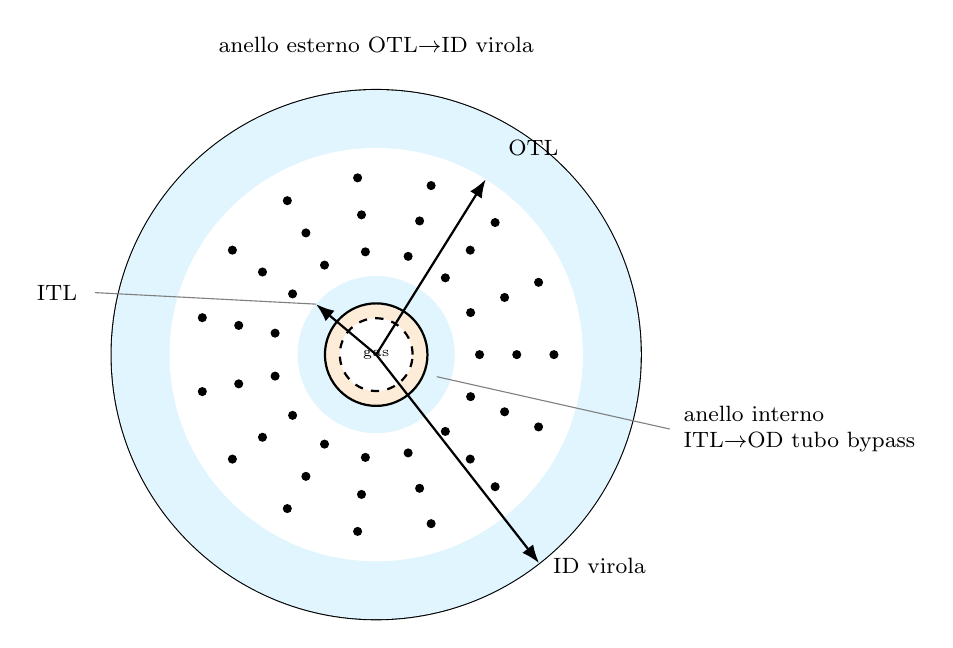
\begin{tikzpicture}[scale=1.05]
\draw[thick] (0,0) circle (3.2);
\draw[dashed,thick] (0,0) circle (2.5);
\draw[dashed,thick] (0,0) circle (0.95);
\fill[cyan!12] (0,0) circle (3.2);
\fill[white] (0,0) circle (2.5);
\fill[cyan!12] (0,0) circle (0.95);
% tube field between ITL and OTL
\foreach \r in {1.25,1.7,2.15}{
  \foreach \a in {0,24,...,336}{
    \fill[black] ({\r*cos(\a)},{\r*sin(\a)}) circle (0.055);
  }
}
% central bypass tube with lining
\fill[boxorange] (0,0) circle (0.62);
\fill[white] (0,0) circle (0.44);
\draw[thick] (0,0) circle (0.62);
\draw[thick,dashed] (0,0) circle (0.44);
\node[font=\tiny] at (0,0) {gas};
\draw[-{Latex},thick] (0,0) -- ({0.95*cos(140)},{0.95*sin(140)});
\node[font=\footnotesize,anchor=east] at (-3.5,0.75) {ITL};
\draw[gray] (-3.4,0.75) -- ({0.95*cos(140)},{0.95*sin(140)});
\draw[-{Latex},thick] (0,0) -- ({2.5*cos(58)},{2.5*sin(58)});
\node[font=\footnotesize] at (1.9,2.5) {OTL};
\draw[-{Latex},thick] (0,0) -- ({3.2*cos(-52)},{3.2*sin(-52)});
\node[font=\footnotesize] at (2.7,-2.55) {ID virola};
\node[font=\footnotesize,anchor=west,align=left] at (3.6,-0.9) {anello interno\\ ITL$\to$OD tubo bypass};
\draw[gray] (3.55,-0.9) -- ({0.78*cos(-20)},{0.78*sin(-20)});
\node[font=\footnotesize,align=center] at (0,3.75) {anello esterno OTL$\to$ID virola};
\end{tikzpicture}
\end{document}
